Since the blockchain technology is proposed, different methods for visualization and analysis are explored. As Bitcoin is the first and main blockchain network in the world and the data can be accessed publicly, much literature conducts researches based on it. Generally, there are three categories of related works for the visualization of a blockchain system.
\begin{itemize}
    \item \textbf{Visualization of Blockchain Information} \\
        There are a lot of online visualization applications which can visualize the static information of transactions and blocks on a blockchain system. They display the information in detail and usually serve as the base for analysis.
    \item \textbf{Analysis of Bitcoin Transactions} \\
        As Bitcoin becomes a popular peer-to-peer network recently, most of the recent literature focuses on the analysis of the relationships between transactions and blocks on Bitcoin network. They try to recognize special patterns to gain economic experience and prevent criminal activities.
    \item \textbf{Analysis of Consensus Protocols} \\
        An analysis of the consensus protocols on the blockchain networks is an interesting topic as it can reveal the potential applications on blockchain platforms.
\end{itemize}

\section{Visualization of Blockchain Information}

There are some online tools and applications that provide visualization of the static status and information of transactions and blocks on Bitcoin network. Tri A. Sundara et al. \cite{Sundara2017} summarized 8 visualization applications and compared their visualization methods and technologies. We shortly review these applications here, so the main difference between our application and them can be identified clearly.
\clearpage

\begin{itemize}
    \item \textbf{Bitbonkers} \cite{bitbonkers} \\
        Bitbonkers rendered a live 3D animation of transactions and blocks. Balls represent transactions, and they keep dropping down to the plate from the top. On the other hand, cubics represent blocks. The sizes of balls are different according to their total values. (Figure \ref{fig:bitbonkers})
        \begin{figure}[htb]
            \centering
            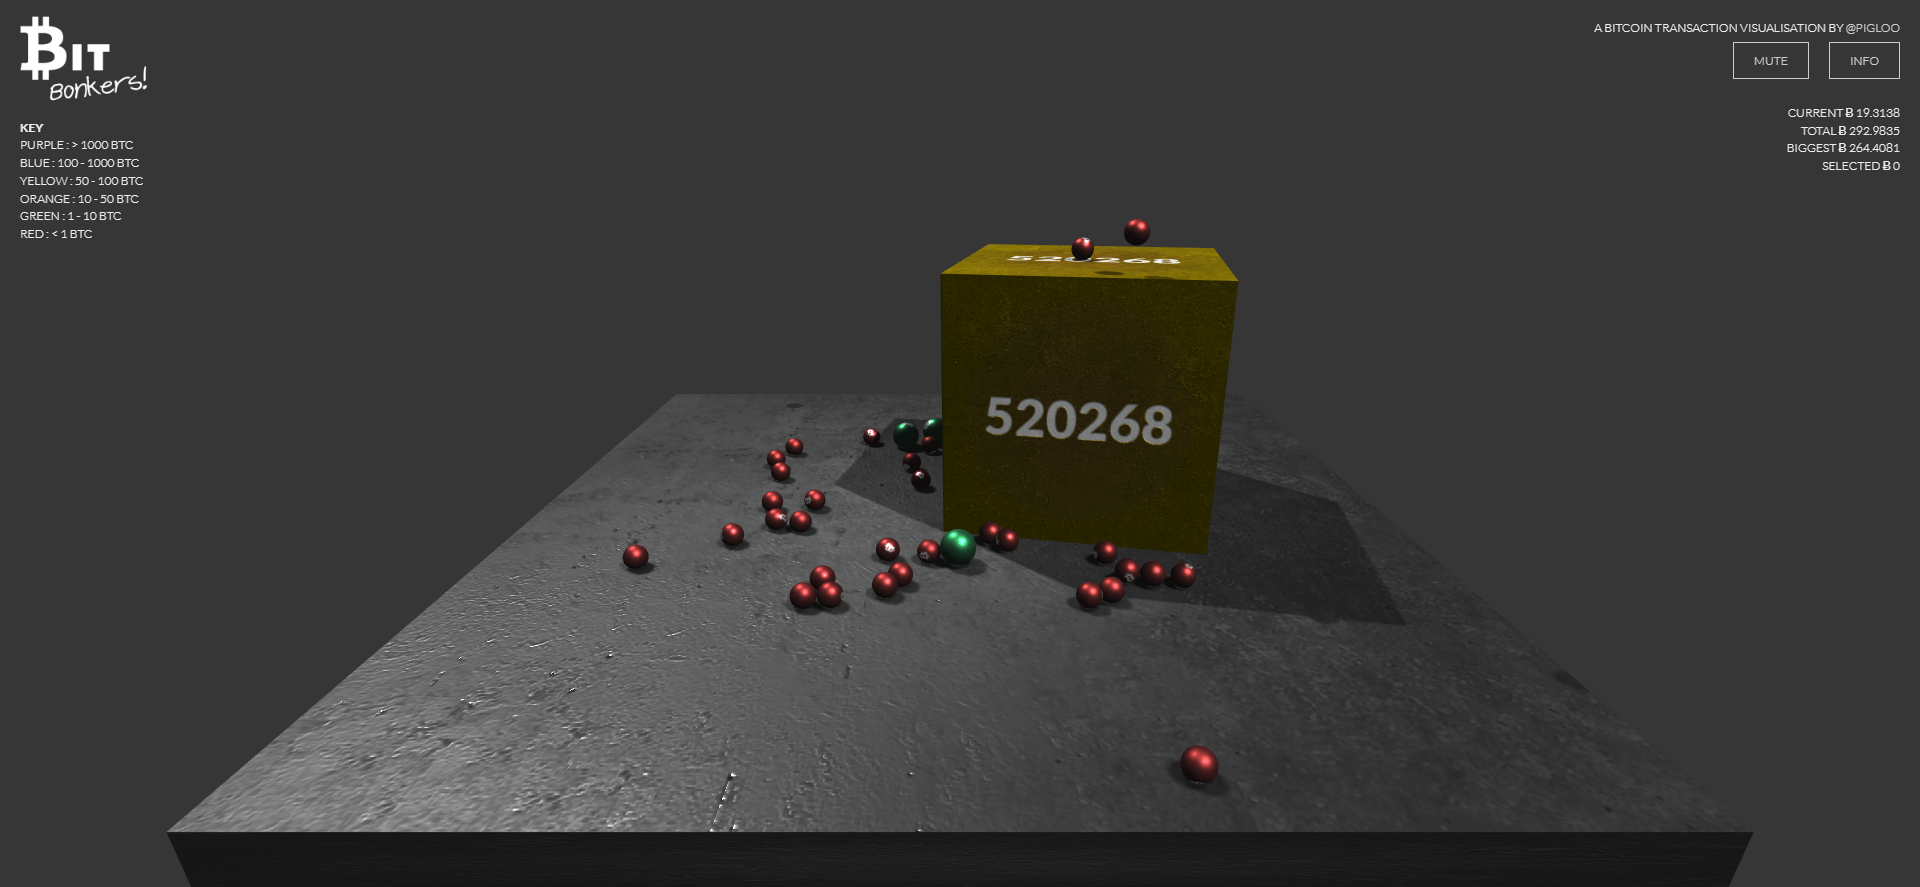
\includegraphics[width=\textwidth]{related_bitbonkers}
            \caption{Bitbonkers.}
            \label{fig:bitbonkers}
        \end{figure}
    \item \textbf{Bitnodes} \cite{bitnodes} \\
        Bitnodes focused on the visualization of the distribution of nodes on Bitcoin network. The density of nodes indicates the most active areas on Bitcoin network in the world.(Figure \ref{fig:bitnodes})
        \begin{figure}[htb]
            \centering
            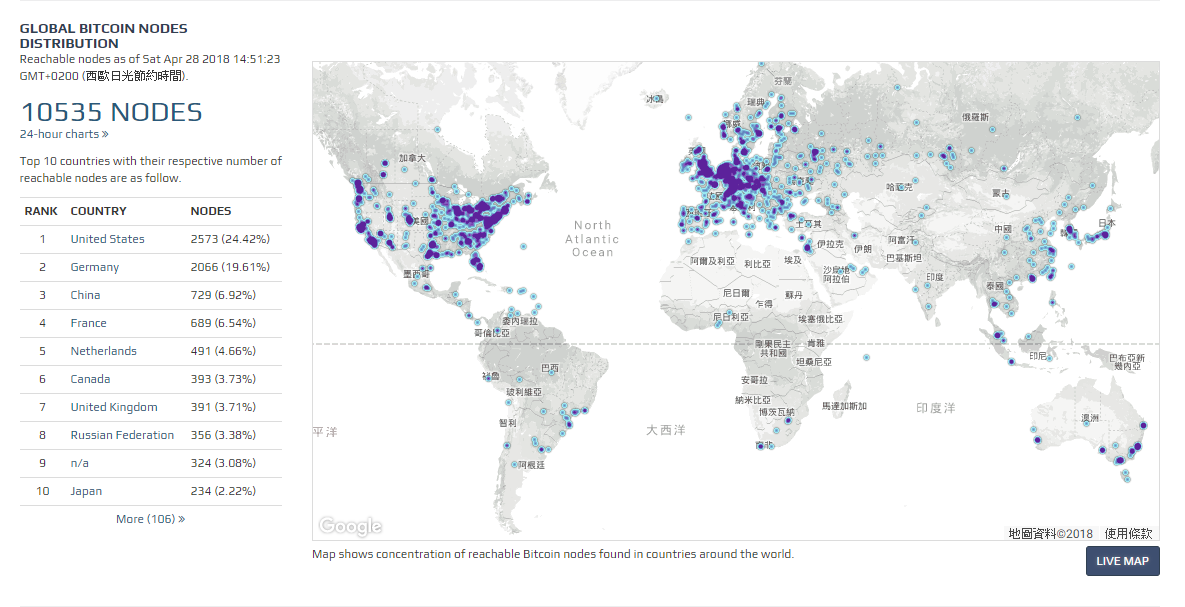
\includegraphics[width=\textwidth]{related_bitnodes}
            \caption{Bitnodes.}
            \label{fig:bitnodes}
        \end{figure}
    \clearpage
    \vspace*{\fill}
    \item \textbf{BitcoinCity} \cite{bitcoincity} \\
        BitcoinCity built a small city as the visualization of Bitcoin. It used a road to chain the blocks, and the houses with different heights on both sides of the road represented transactions with different values. (Figure \ref{fig:bitcoincity})
        \begin{figure}[htb]
            \centering
            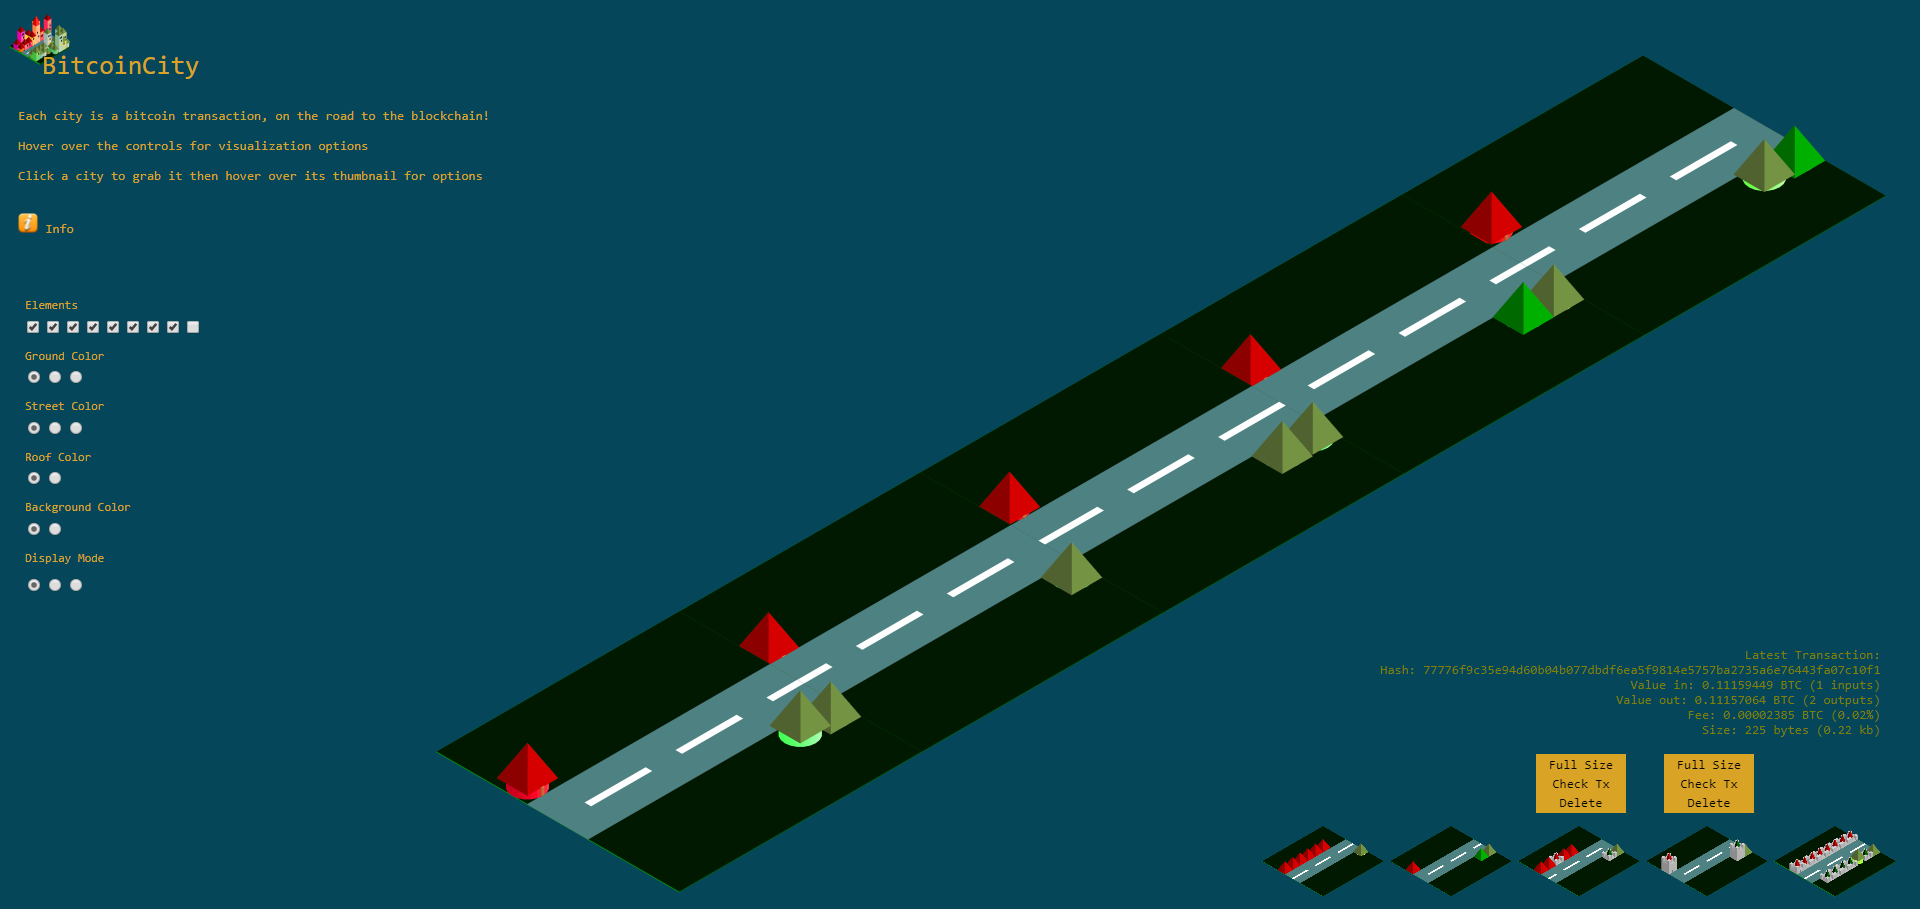
\includegraphics[width=\textwidth]{related_bitcoincity}
            \caption{BitcoinCity.}
            \label{fig:bitcoincity}
        \end{figure}
    \item \textbf{Blockseer} \cite{blockseer} \\
        Blockseer located a mined transaction and visualized the outputs of the transaction. For example, the screenshot shows there are nine outputs of the transaction which in at the root of the tree structure. That is, the transaction is divided into nine parts which are delivered to different addresses respectively. (Figure \ref{fig:blockseer})
        \begin{figure}[htb]
            \centering
            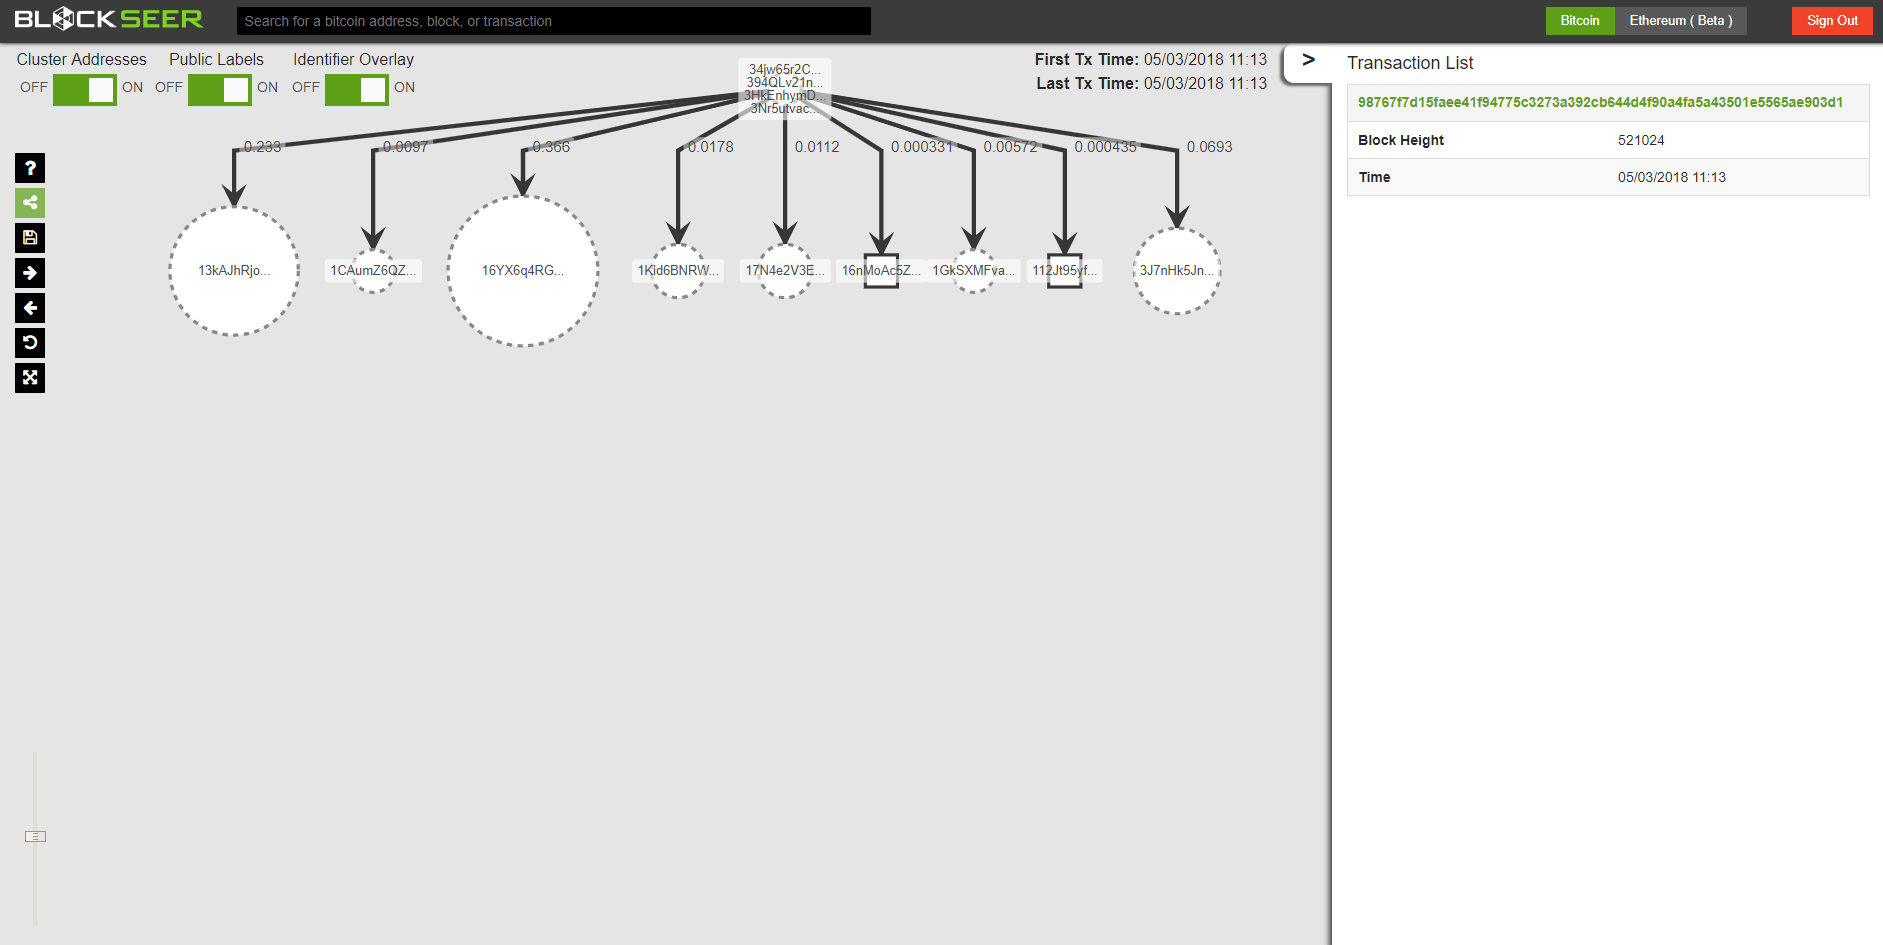
\includegraphics[width=\textwidth]{related_blockseer}
            \caption{Blockseer.}
            \label{fig:blockseer}
        \end{figure}
    \vspace*{\fill}
    \clearpage
    \vspace*{\fill}
    \item \textbf{DailyBlockchain} \cite{dailyblockchain} \\
        DailyBlockchain displayed the mined transactions as the biological cells. The size of the cell are determined by the number of outputs of the transaction. The cells are generated from the center and spread toward every direction. (Figure \ref{fig:dailyblockchain})
        \begin{figure}[htb]
            \centering
            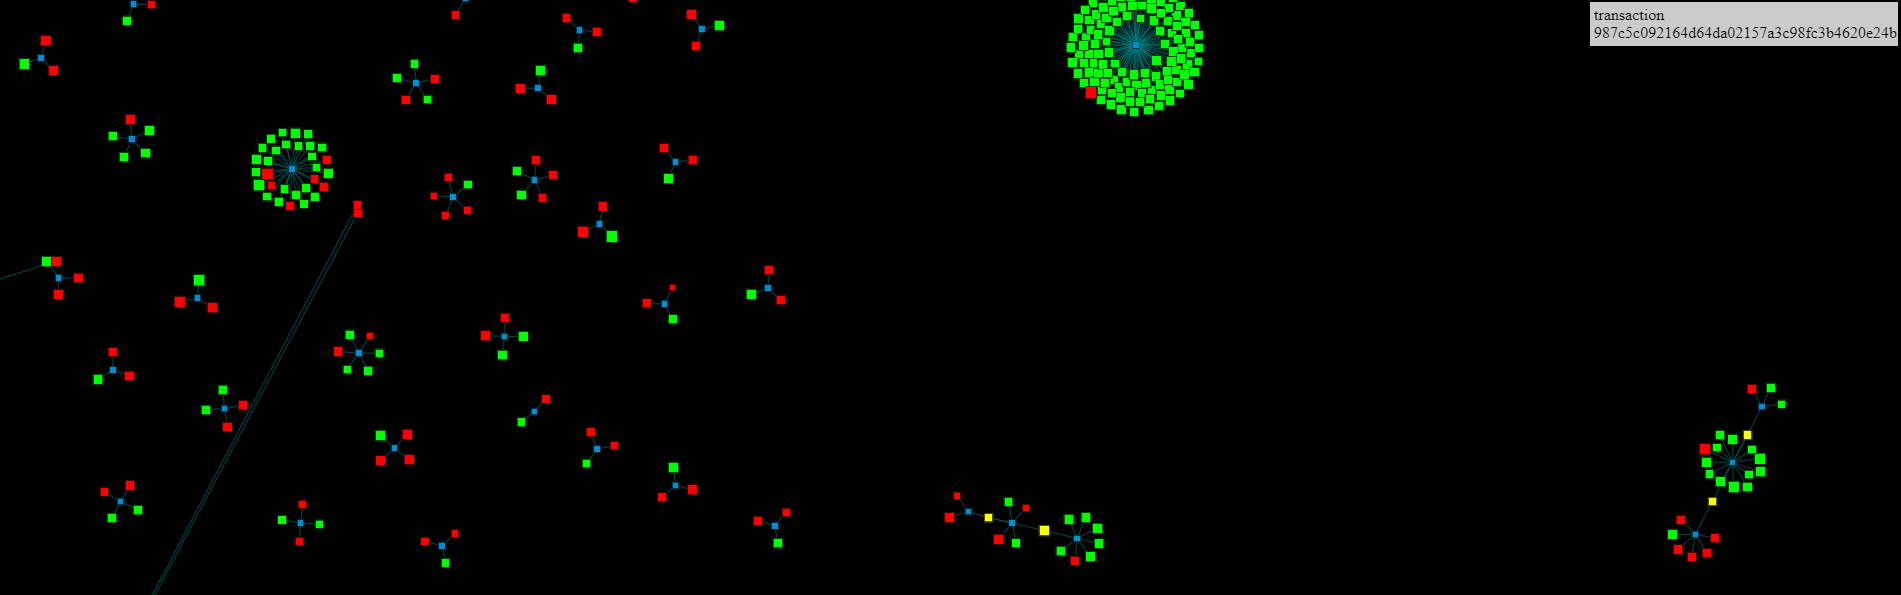
\includegraphics[width=\textwidth]{related_dailyblockchain}
            \caption{DailyBlockchain.}
            \label{fig:dailyblockchain}
        \end{figure}
    \item \textbf{Elliptic} \cite{elliptic} \\
        Elliptic visualized the whole history of Bitcoin like the Big Bang of the universe. However, the oldest blocks are placed at the center of the universe, which is opposite to the Big Bang theory in the reality. The blocks are divided by the dotted circles according to their birth years. (Figure \ref{fig:elliptic})
        \begin{figure}[htb]
            \centering
            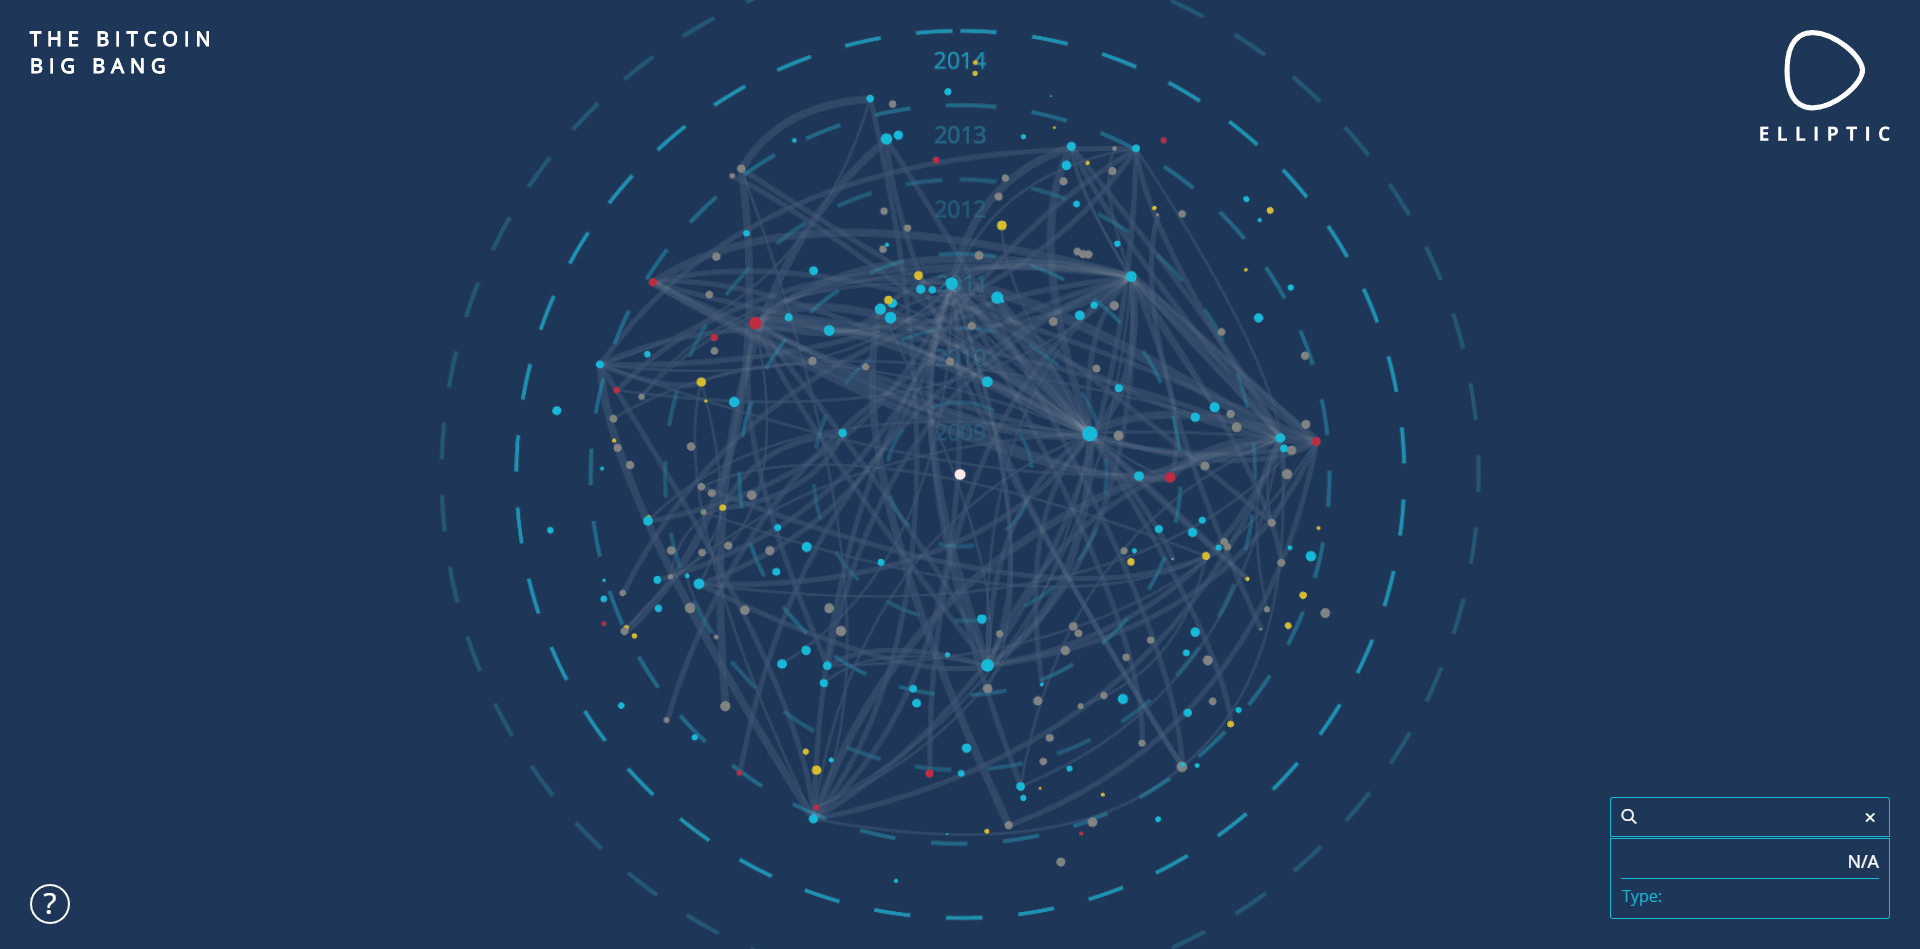
\includegraphics[width=\textwidth]{related_elliptic}
            \caption{Elliptic.}
            \label{fig:elliptic}
        \end{figure}
    \vspace*{\fill}
    \clearpage
    \item \textbf{Interaqt} \cite{interaqt} \\
        Interaqt gathered the mined transactions which are represented in circles into a big circle. The screen is empty at first, the more and more transactions will join into the big circle as time passes. (Figure \ref{fig:interaqt})
        \begin{figure}[htb]
            \centering
            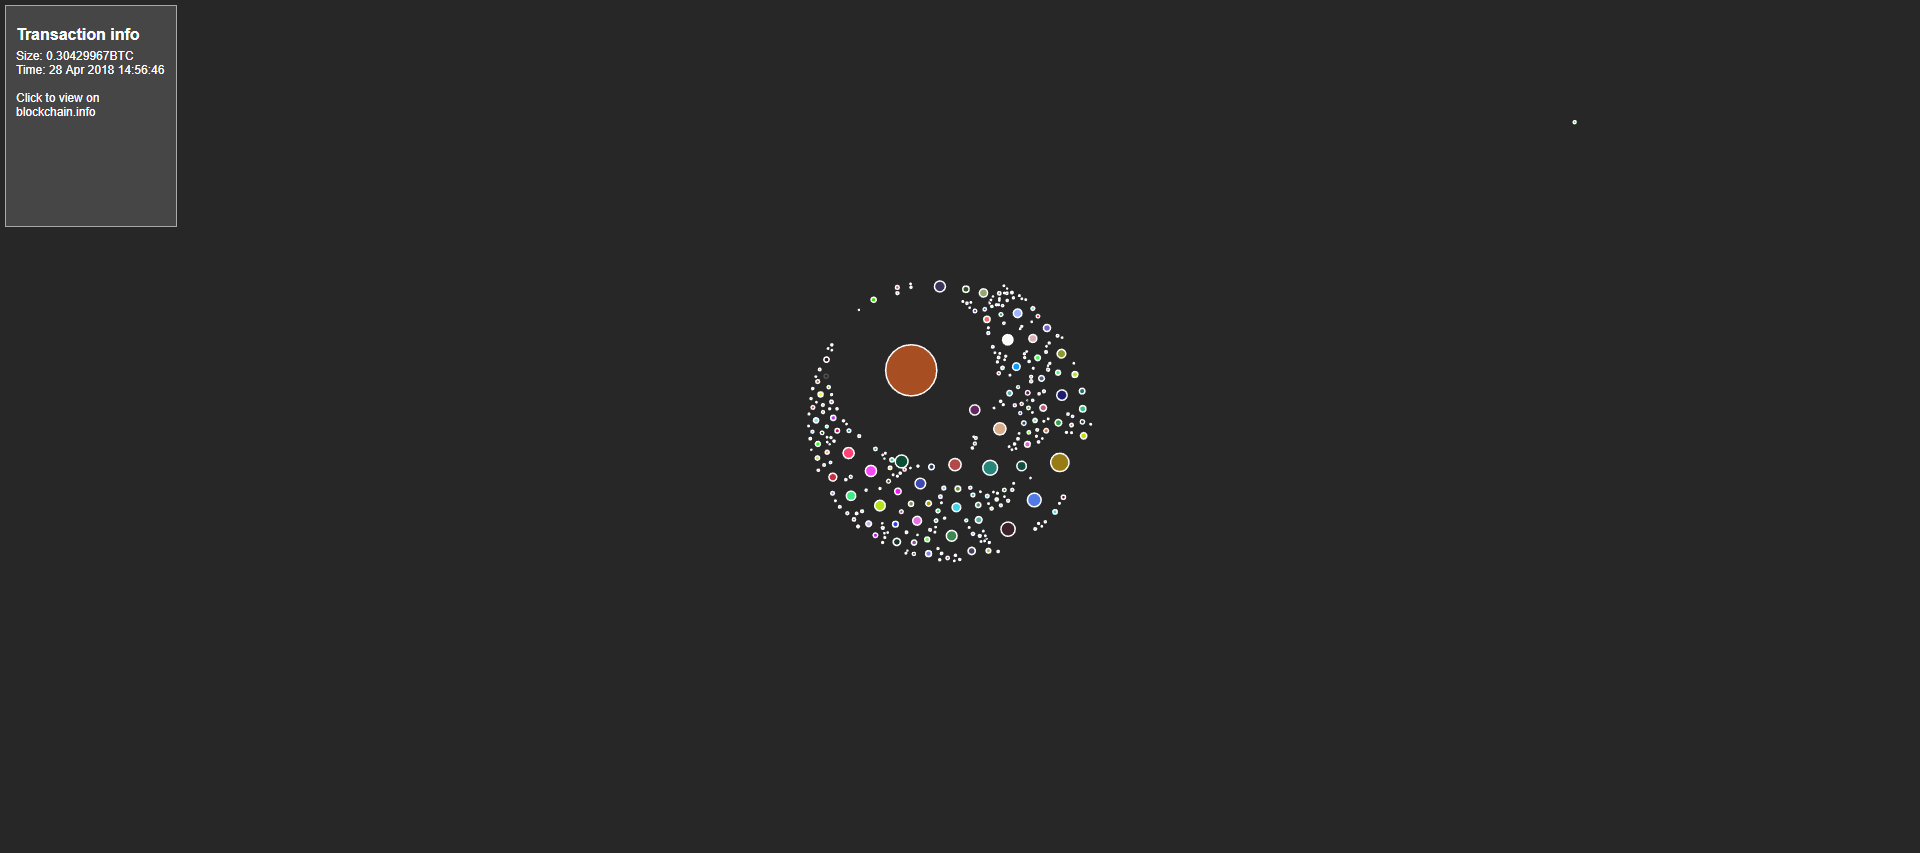
\includegraphics[width=\textwidth]{related_interaqt}
            \caption{Interaqt.}
            \label{fig:interaqt}
        \end{figure}
    \item \textbf{Live Globe} \cite{liveglobe} \\
        Live Globe combined the geographies of blocks and the earth together in the visualization. There are two blocks that are placed at the position of New York City in the screenshot. However, the color of the blocks are also green, so it is difficult to distinguish them. (Figure \ref{fig:live globe})
        \begin{figure}[htb]
            \centering
            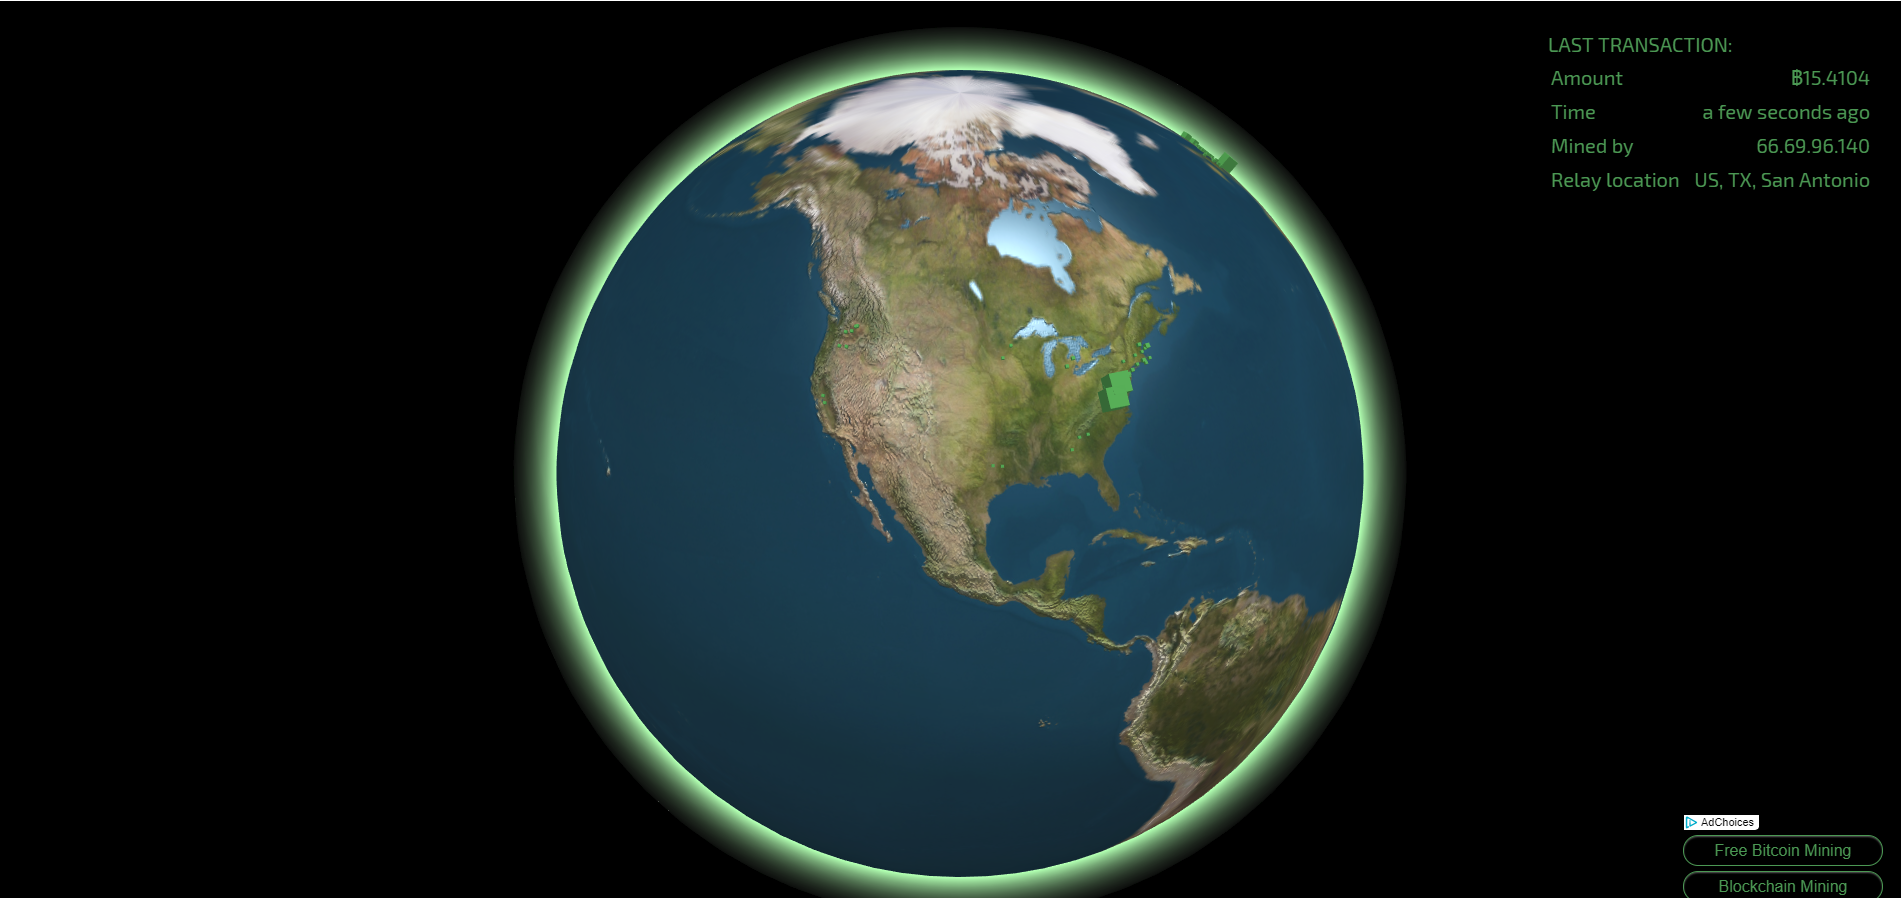
\includegraphics[width=\textwidth]{related_liveglobe}
            \caption{Live Globe.}
            \label{fig:live globe}
        \end{figure}
\end{itemize}

\clearpage

In addition to the 2D and 3D animations of the visualization of Bitcoin, there are applications which use tabular methods as the visualization of blockchains.

\begin{itemize}
    \item \textbf{Blockchain} \cite{blockchain} \\
        The tabular (Figure \ref{fig:blocks by blockchain}) contains the height, the timestamp, the mined transactions, the total values, the size, etc. of mined blocks on Bitcoin network. The details information of a block can be viewed by selecting it, and then the list of included transactions with addresses, inputs, and outputs (Figure \ref{fig:transactions by blockchain}) is displayed.

        \begin{figure}[htb]
            \centering
            \begin{subfigure}[b]{1\textwidth}
                \centering
                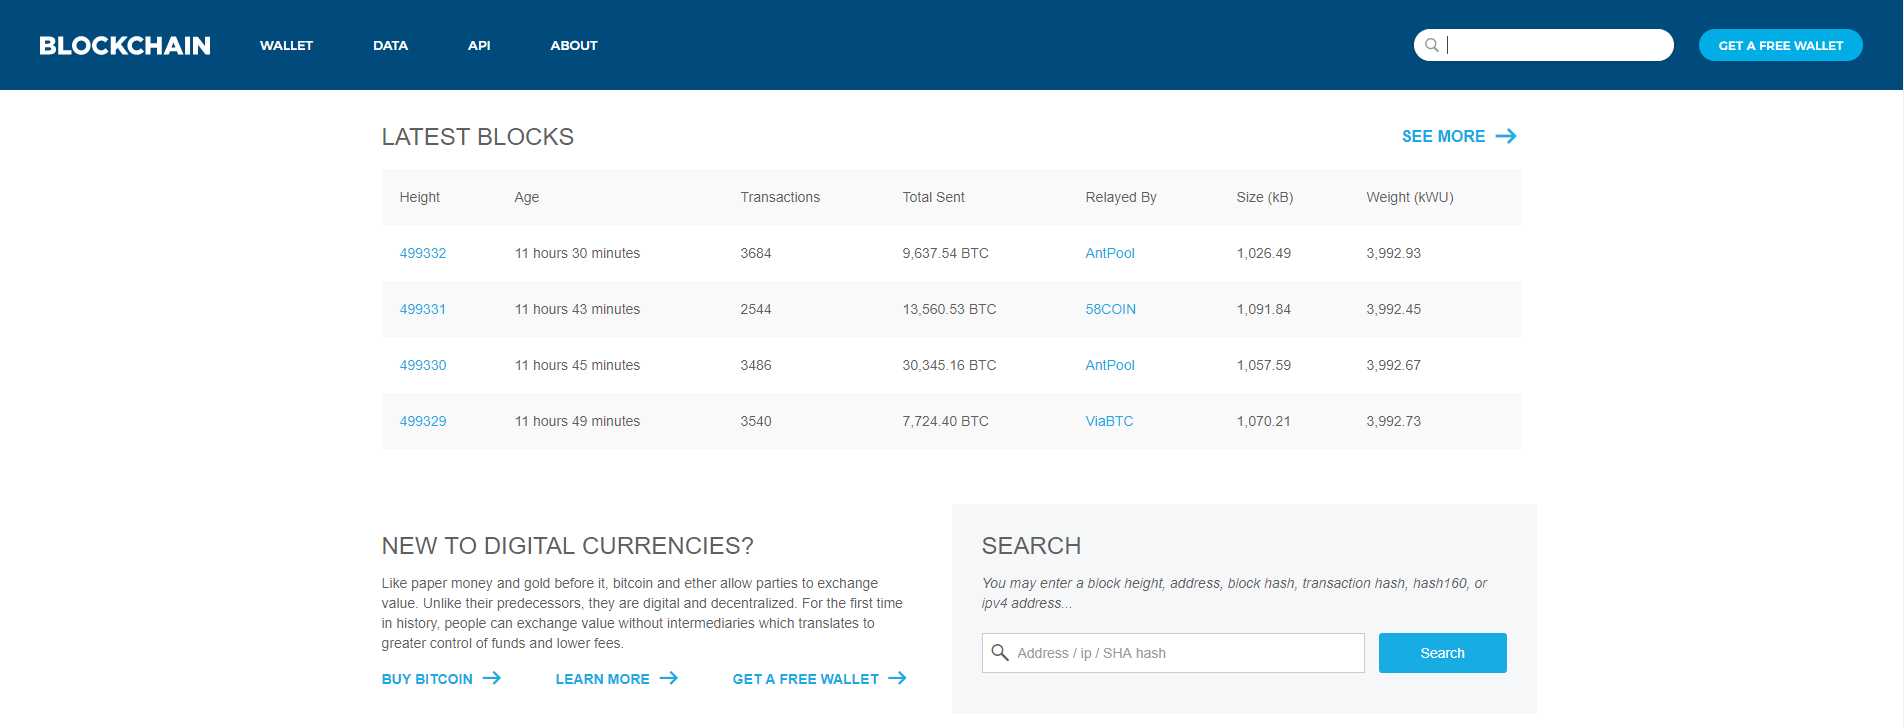
\includegraphics[width=\textwidth]{related_blockchain}
                \caption{Blocks by Blockchain.}
                \label{fig:blocks by blockchain}
            \end{subfigure}

            \begin{subfigure}[b]{1\textwidth}
                \centering
                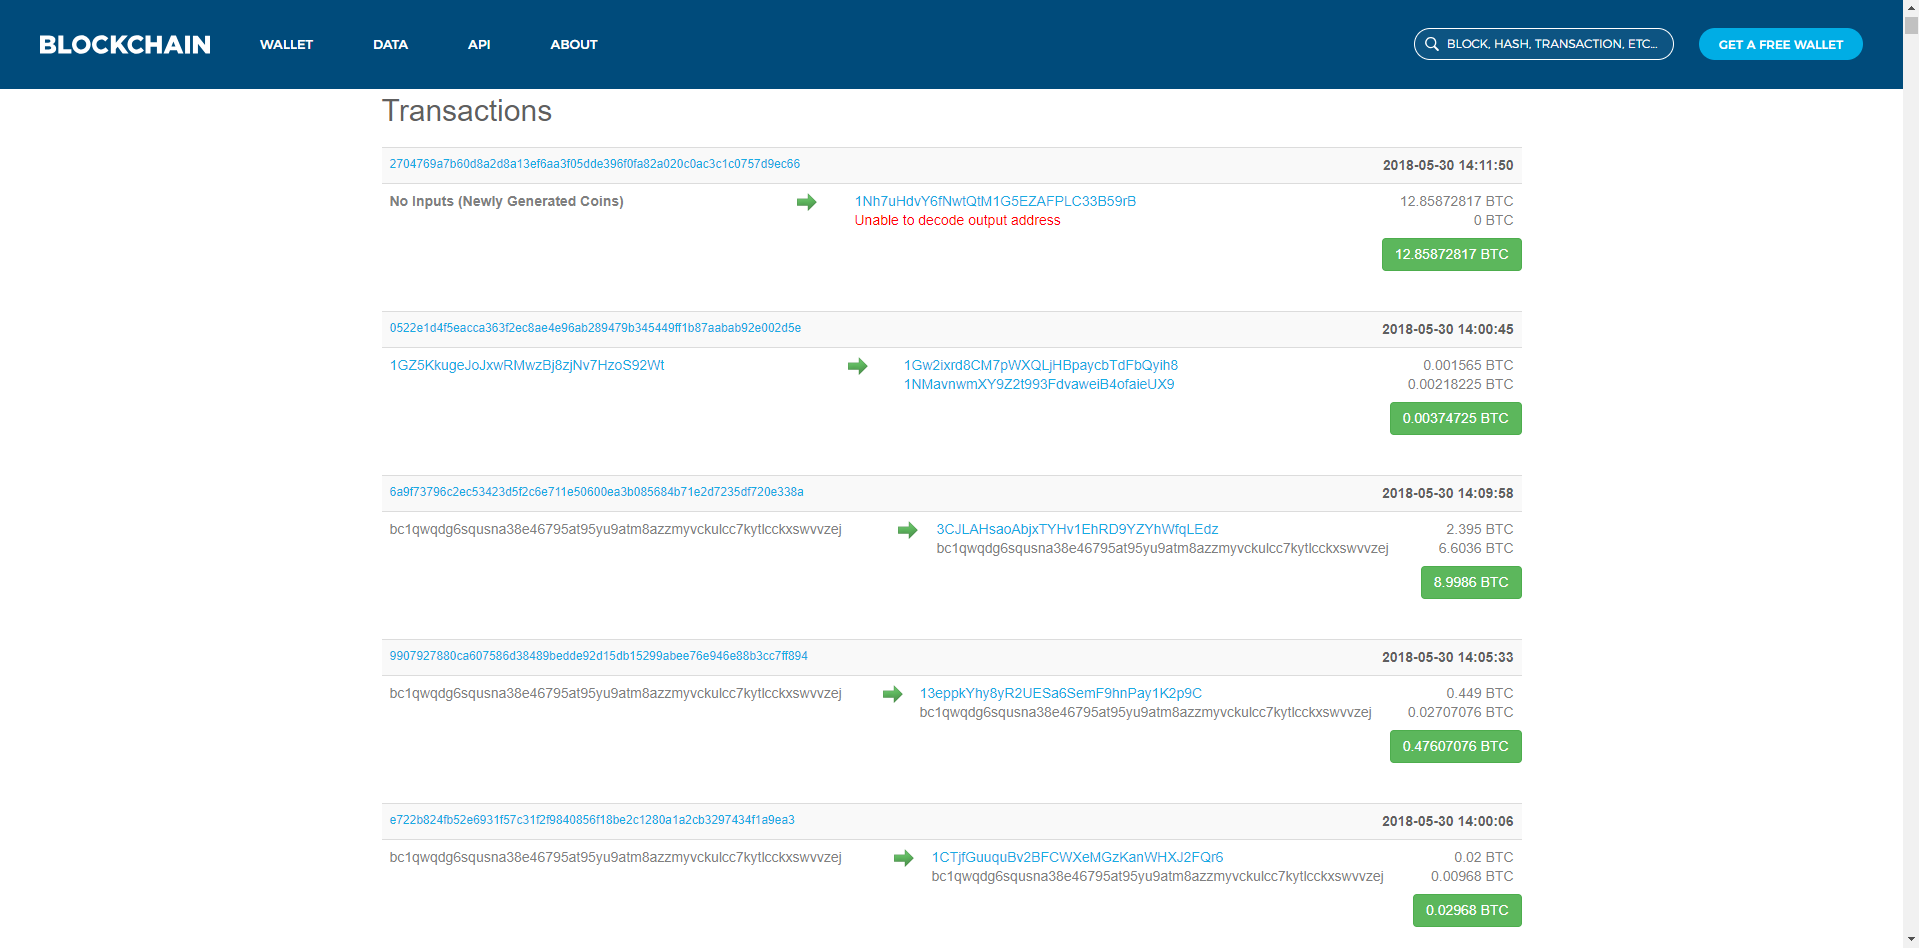
\includegraphics[width=\textwidth]{related_blockchain2}
                \caption{Transactions by Blockchain}
                \label{fig:transactions by blockchain}
            \end{subfigure}

            \caption{Blockchain.}
        \end{figure}
    \item \textbf{Etherscan} \cite{etherscan} \\
        Etherscan which is for Ethereum network is similar to Blockchain, but it places the information of blocks and transactions in the same page. The top right part displays the line chart of the marketing value of Ethereum. The list of blocks is placed on the bottom left of the page, and the list of transactions is at the bottom right part. The details can also be checked by selecting individual blocks or transactions. (Figure \ref{fig:etherscan})
        \begin{figure}[htb]
            \centering
            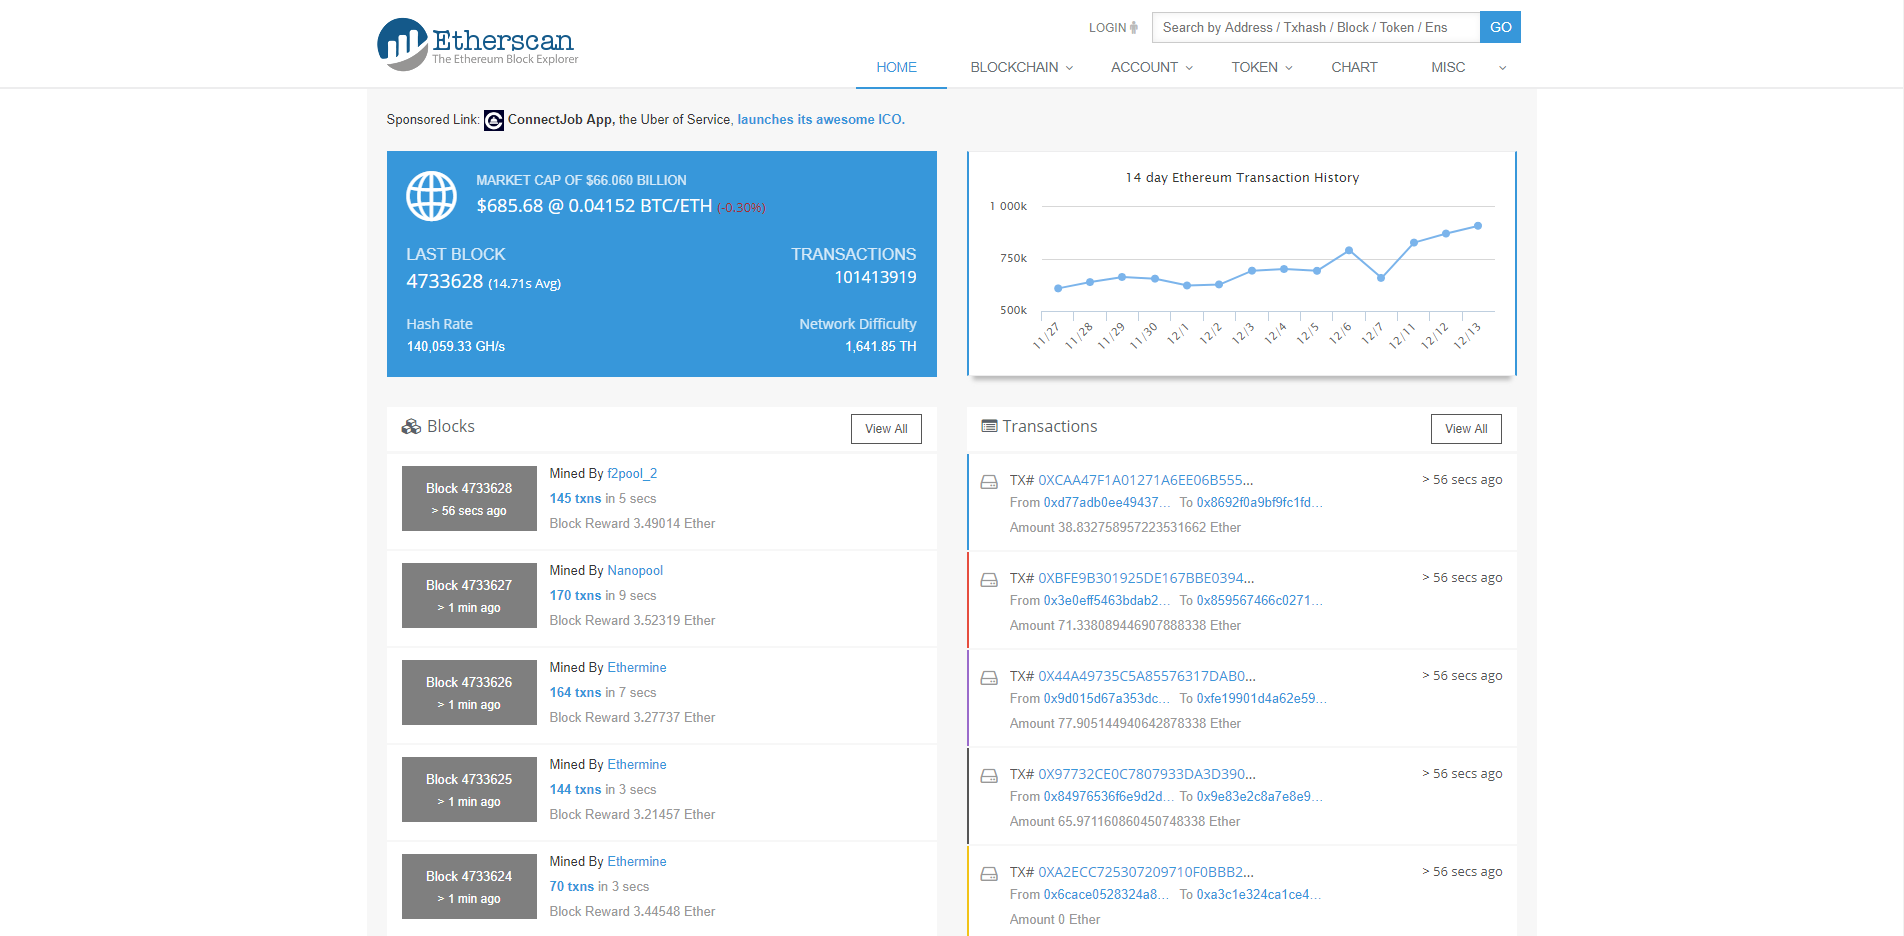
\includegraphics[width=\textwidth]{related_etherscan}
            \caption{Etherscan.}
            \label{fig:etherscan}
        \end{figure}
\end{itemize}

In short conclusion, although the above tools and applications showed visualization methods of blockchains, their goals are to provide the static information and statistics instead of the dynamic mining processes that happen in a blockchain system. It is difficult to gain valuable understandings about the complex and dynamic mining processes in these applications.

\section{Analysis of Bitcoin Transactions}

As Bitcoin is the most popular and famous blockchain network currently, it is worth to explore the patterns of transactions and blocks to prevent malicious abuse of blockchain services. The nodes and transactions are anonymous on blockchain networks, so the recognition of patterns can be challengeable. Here we present some analysis methods and visualization technologies that can identify the relationships between nodes and transactions in time series on Bitcoin network.

\clearpage

\begin{itemize}
    \item \textbf{BitConeView: Visualization of Flows in the Bitcoin Transaction Graph} \cite{Battista2015} \\
        Giuseppe Di Battista et al. provided a visualization tool called \textit{BitConeView} that analyzed the flows of bitcoins in the transactions by timestamps. It can be used to analyze the patterns of the flows of bitcoins and locate tainted transactions. Figure \ref{fig:bitconeview} \cite{Battista2015} shows that the flows of bitcoins are visualized in time series, and the lifetime of a bitcoin can be tracked in the connected bars which are blocks.
        \begin{figure}[htb]
            \centering
            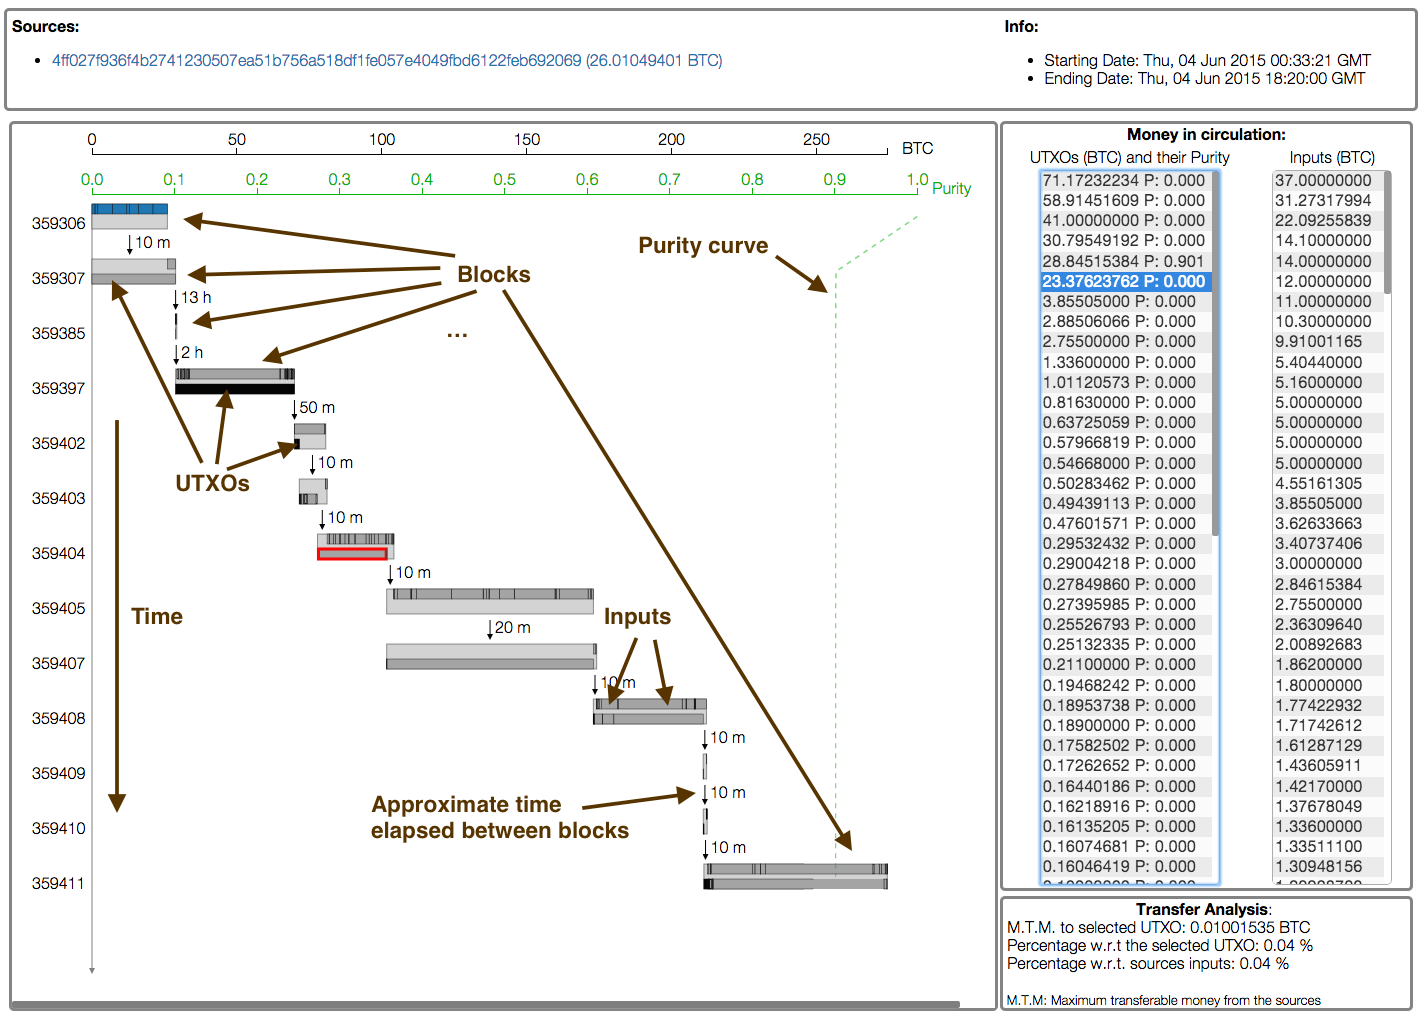
\includegraphics[width=0.6\textwidth]{related_bitconeview}
            \caption{BitConeView.}
            \label{fig:bitconeview}
        \end{figure}
    \item \textbf{Blockchain Explorer: An Analytical Process and Investigation Environment for Bitcoin} \cite{Kuzuno2017} \\
        To prevent the criminal activities and illegal behaviors that abuse the services of Bitcoin, Hiroki Kuzuno et al. proposed an analyzing system which managed the data and statistics of blockchains for the usages of law enforcement investigation and training. 
        Figure \ref{fig:analysis methods by blockchain explorer} \cite{Kuzuno2017} shows the analysis methods in the visualization. The line chart on the left side represents the balance of an address, and the bar charts on the right side represent the number of transactions in hours or weeks.
        \begin{figure}[htb]
            \centering
            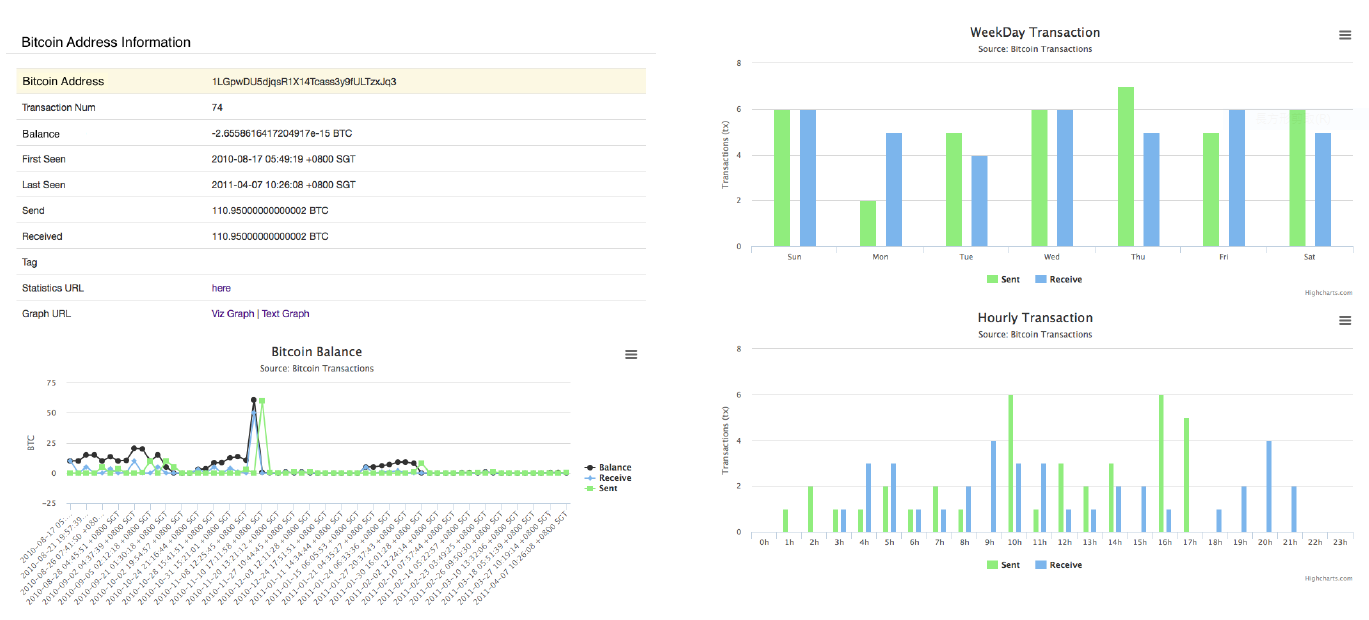
\includegraphics[width=0.7\textwidth]{related_blockchain_explorer}
            \caption{Analysis methods by Blockchain Explorer.}
            \label{fig:analysis methods by blockchain explorer}
        \end{figure}
        \clearpage
        Figure \ref{fig:activities of an address by blockchain explorer} \cite{Kuzuno2017} displays the activities of an address in calendars. The bright squares indicate the time when the address published transactions.
        \begin{figure}[htb]
            \centering
            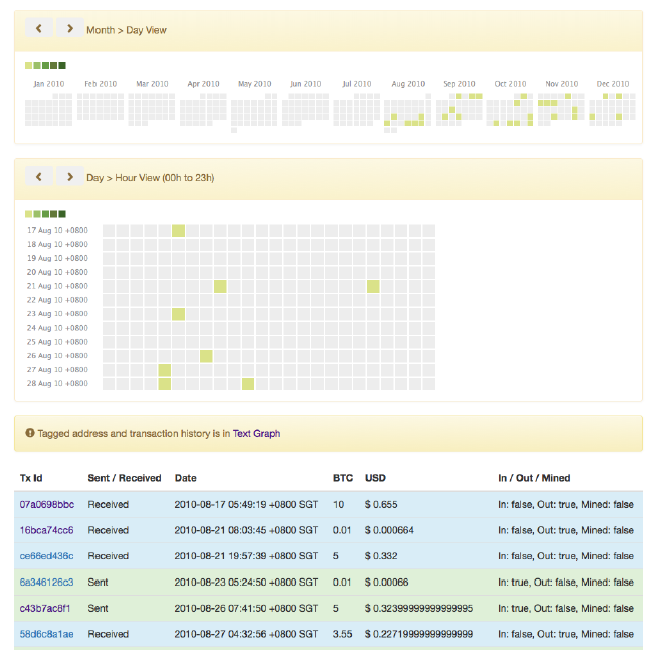
\includegraphics[width=0.6\textwidth]{related_blockchain_explorer2}
            \caption{Activities of an address by Blockchain Explorer.}
            \label{fig:activities of an address by blockchain explorer}
        \end{figure}

        Figure \ref{fig:mappings of inputs and outputs in a transaction bblockchain explorer} \cite{Kuzuno2017} maps the inputs and outputs of a transaction into tree structures. As a result, the flows of bitcoins can be tracked by the input and output nodes. 
        \begin{figure}[htb]
            \centering
            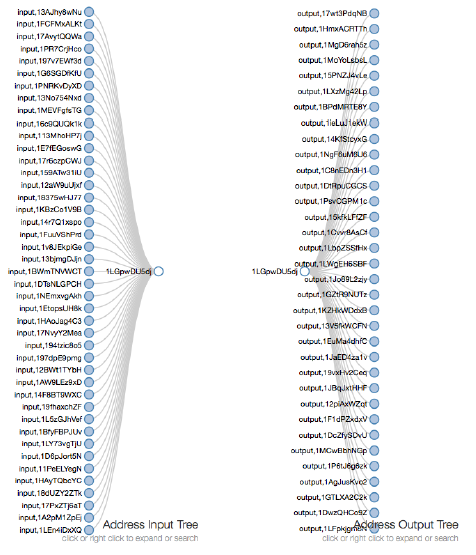
\includegraphics[width=0.4\textwidth]{related_blockchain_explorer3}
            \caption{Mappings of inputs and outputs in a transaction by Blockchain Explorer.}
            \label{fig:mappings of inputs and outputs in a transaction bblockchain explorer}
        \end{figure}

        With above visualization, the activities of an address and the mappings to the real identification can be explored.
        \clearpage
    \item \textbf{Visualizing Dynamic Bitcoin Transaction Patterns} \cite{McGinn2016} \\
        Dan McGinn et al. focused on visualizing transactions of Bitcoin from the top-down viewpoint. The visualization of the large scale of data provided domain experts and the general public a tool to analyze and identify the transaction patterns with big data visualization methods. Figure \ref{fig:visualization by dan mcGinn et al} \cite{McGinn2016} shows the visualization result. The blocks are connected by lines if they contain related transactions. Thus, different patterns can be identified in the graphs.
        \begin{figure}[htb]
            \centering
            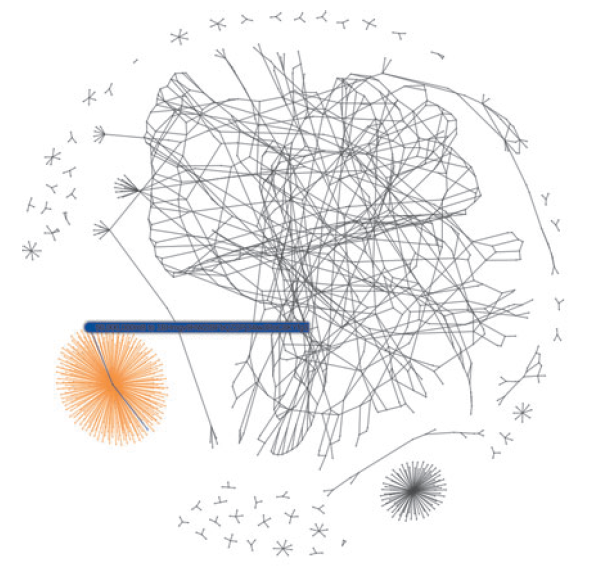
\includegraphics[width=0.4\textwidth]{related_McGinn}
            \caption{Visualization by Dan McGinn et al.}
            \label{fig:visualization by dan mcGinn et al}
        \end{figure}
    \item \textbf{Bitcoin Visualization} \cite{Saublet2015} \\
        The visual analytics tool that was proposed by Loïs Saublet enabled economists to analyze the metrics and actors on Bitcoin network and provided good user experience by working together with end users. As in Figure \ref{fig:visualization by loïs saublet} \cite{Saublet2015} shows, a period of Bitcoin marketing values can be displayed by a line chart, and economists can examine it.
        \begin{figure}[htb]
            \centering
            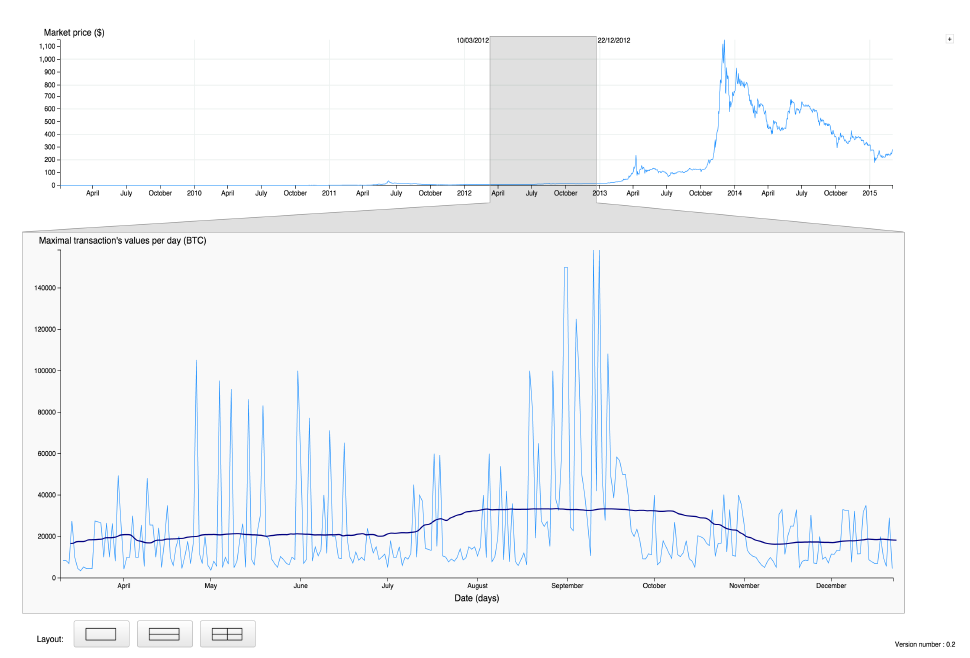
\includegraphics[width=0.8\textwidth]{related_Saublet}
            \caption{Visualization by Loïs Saublet.}
            \label{fig:visualization by loïs saublet}
        \end{figure}
    \item \textbf{Bitcoin Transaction Graph Analysis} \cite{Fleder2015} \\
        Michael Fleder et al. proposed a graph-analysis framework that could analyze the relationships between public addresses and transactions. It can be used to match candidate Bitcoin transactions with the transactions in the reality. As a result, it demonstrated that the transactions are not entirely anonymous on Bitcoin network. Figure \ref{fig:visualization of the transaction graph} \cite{Fleder2015} shows the transaction graph which gathers the data in a whole day. The relationships of transactions can be identified via the connections. The thichness of the lines are the values, so several patterns such as large volume transactions can be analyzed.
        \begin{figure}[htb]
            \centering
            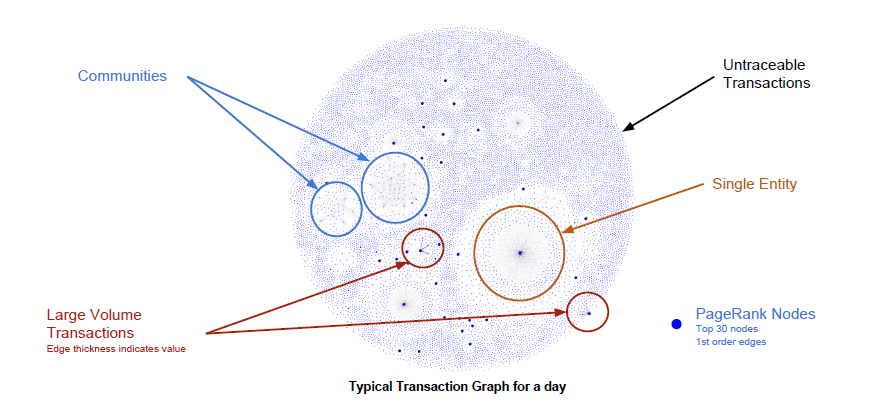
\includegraphics[width=0.8\textwidth]{related_Fleder}
            \caption{Visualization of the transaction graph.}
            \label{fig:visualization of the transaction graph}
        \end{figure}
    \item \textbf{Exploring the Bitcoin Network} \cite{Baumann2014} \\
        The method proposed by Annika Baumann et al. employed graph mining algorithms to analyze the relationship of network usage and exchange rate. It served as the basis for the analysis of the anonymity and economic relationships on Bitcoin network. They used statistical bar charts or line charts for visualization as Figure \ref{fig:visualization by annika baumann et al} \cite{Baumann2014} shows.
        \begin{figure}[htb]
            \centering
            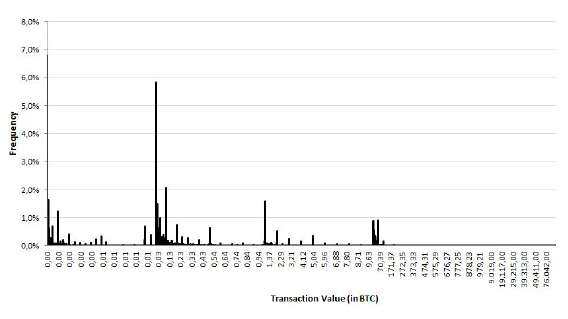
\includegraphics[width=0.8\textwidth]{related_Baumann}
            \caption{Visualization by Annika Baumann et al.}
            \label{fig:visualization by annika baumann et al}
        \end{figure}
\end{itemize}

In summary, the goals of the above tools and methods are to analyze the patterns and relationships of transactions and blocks. That is, they try to recognize patterns to prevent criminal activities and obtain economic inspiration. Therefore, the visualization results of the above literature are more like statistical results for the analysis instead of the mining processes.

\section{Analysis of Consensus Protocols}

To analyze the network conditions of proof-of-work based blockchain system, Amitai Porat et al. \cite{Porat} provided an application that was based on Ethereum platform. It simulates the asynchronous mining activities and network latency, and provided a real-time analysis of the blockchain system. They presented the potential applications of the blockchain technology through the analysis.

Figure \ref{fig:visualization by amitai porat et al} \cite{Porat} shows the visualization by Amitai Porat et al. The visualization is very simple, as the blocks are chained by lines. Therefore, the miners of the blocks cannot be identified in the visualization.

\begin{figure}[htb]
    \centering
    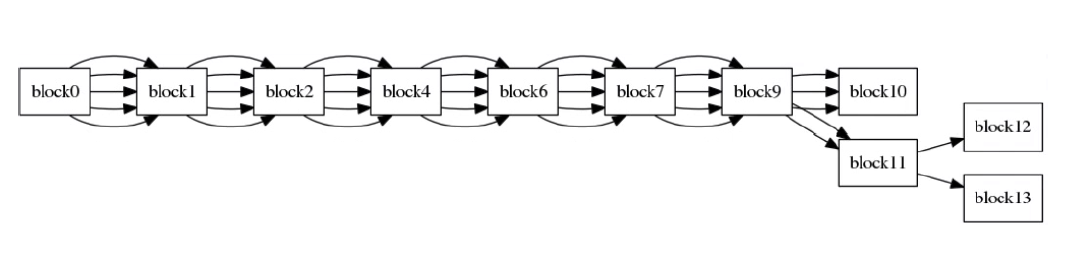
\includegraphics[width=0.8\textwidth]{related_Porat}
    \caption{Visualization by Amitai Porat et al.}
    \label{fig:visualization by amitai porat et al}
\end{figure}

The main difference to our work is that we assume that miners have individual mining strategies which are parameterized, e.g., they select different sets of transactions from transaction pools. Therefore, there are miners who are able to mine blocks faster than the others under the same computing power, but they may suffer lower mining rewards. The combination of different mining strategies and the network delay makes the visualization of the blockchain system dynamic and undetermined. Thus our solution is suitable for researchers to find the influences of different factors on the blockchain system. Moreover, their work focused on finding the potential applications of Ethereum platform. On the other hand, our work emphasize on visualizing the continuous mining processes while miners have different mining strategies and suffer from the network delay. 

\section{Our Approach}

To focus on the dynamic mining activities, our tool provides a real-time visualization of the mining processes that cannot be achieved by the above visualization tools and applications. Through our visualization, users can observe the mining processes step by step. Moreover, our visualization is independent to specific blockchain platforms, e.g., Bitcoin and Ethereum, because we built a simple simulation of the blockchain system ourselves. Therefore, we can concentrate on the mining processes which are the most important activities in a proof-of-work based blockchain system.

\begin{figure}[htb]
    \centering
    \begin{subfigure}[b]{1\textwidth}
        \centering
        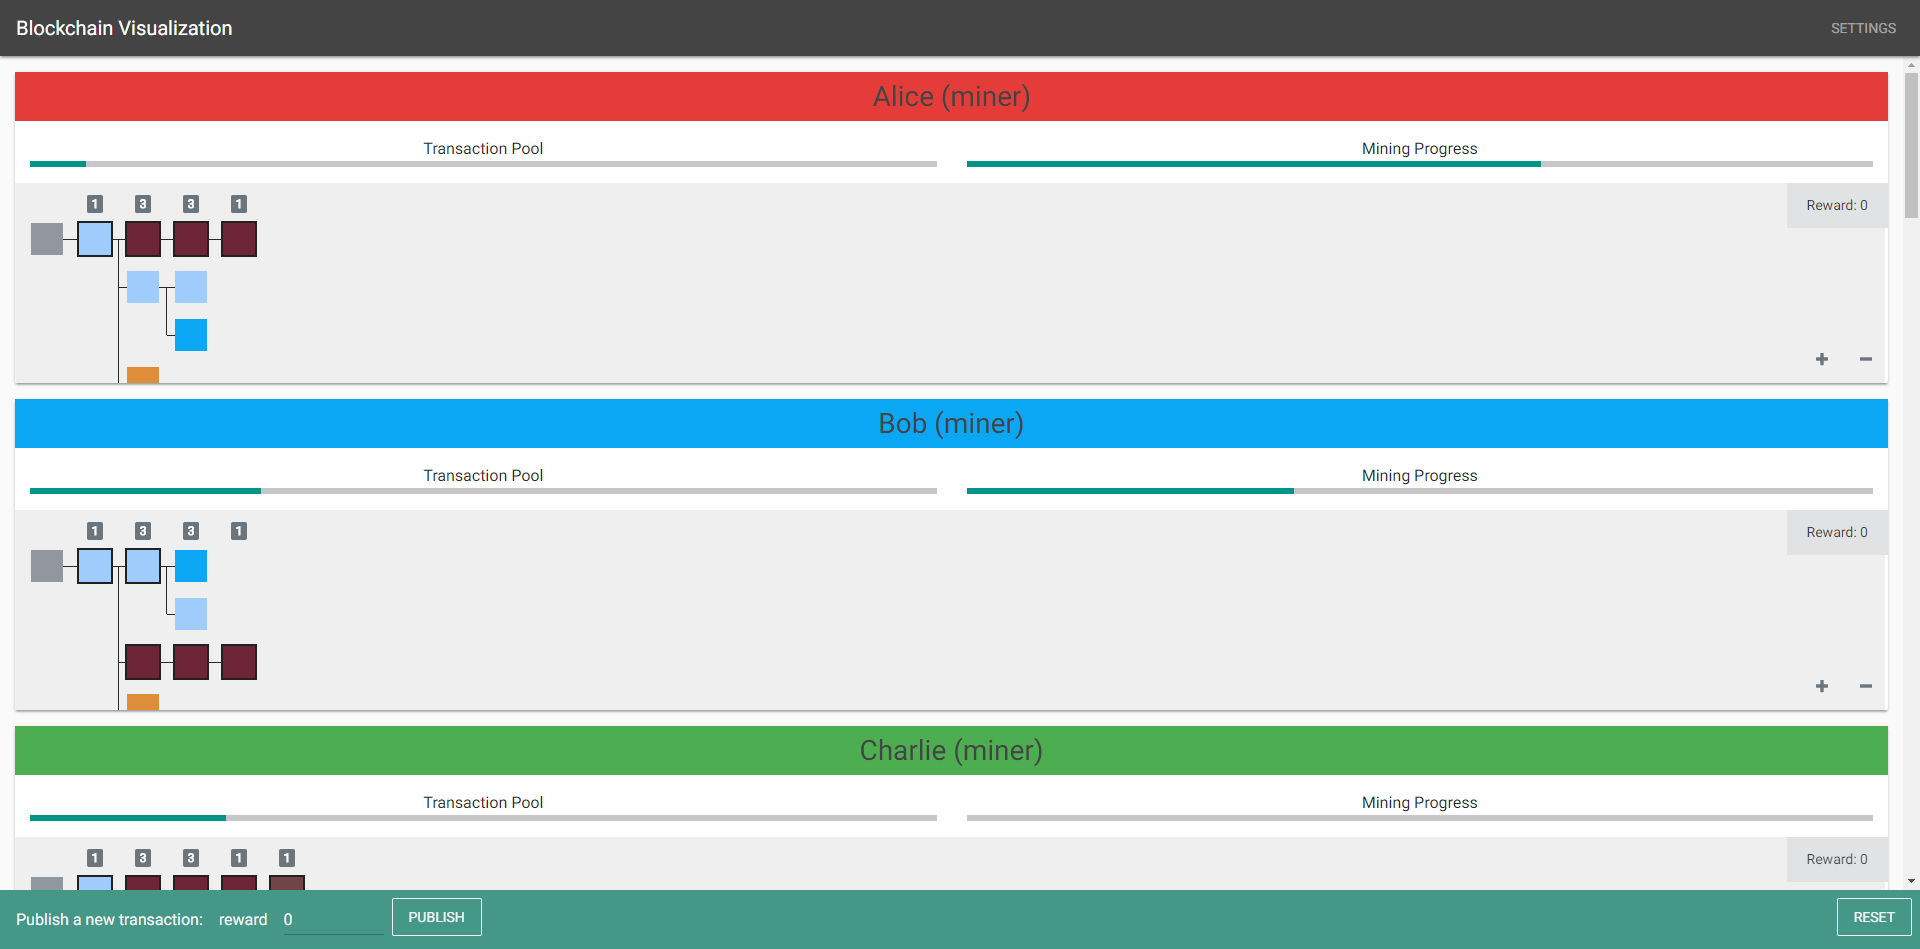
\includegraphics[width=\textwidth]{related_us1}
        \caption{Mining Step 1}
    \end{subfigure}

    \begin{subfigure}[b]{1\textwidth}
        \centering
        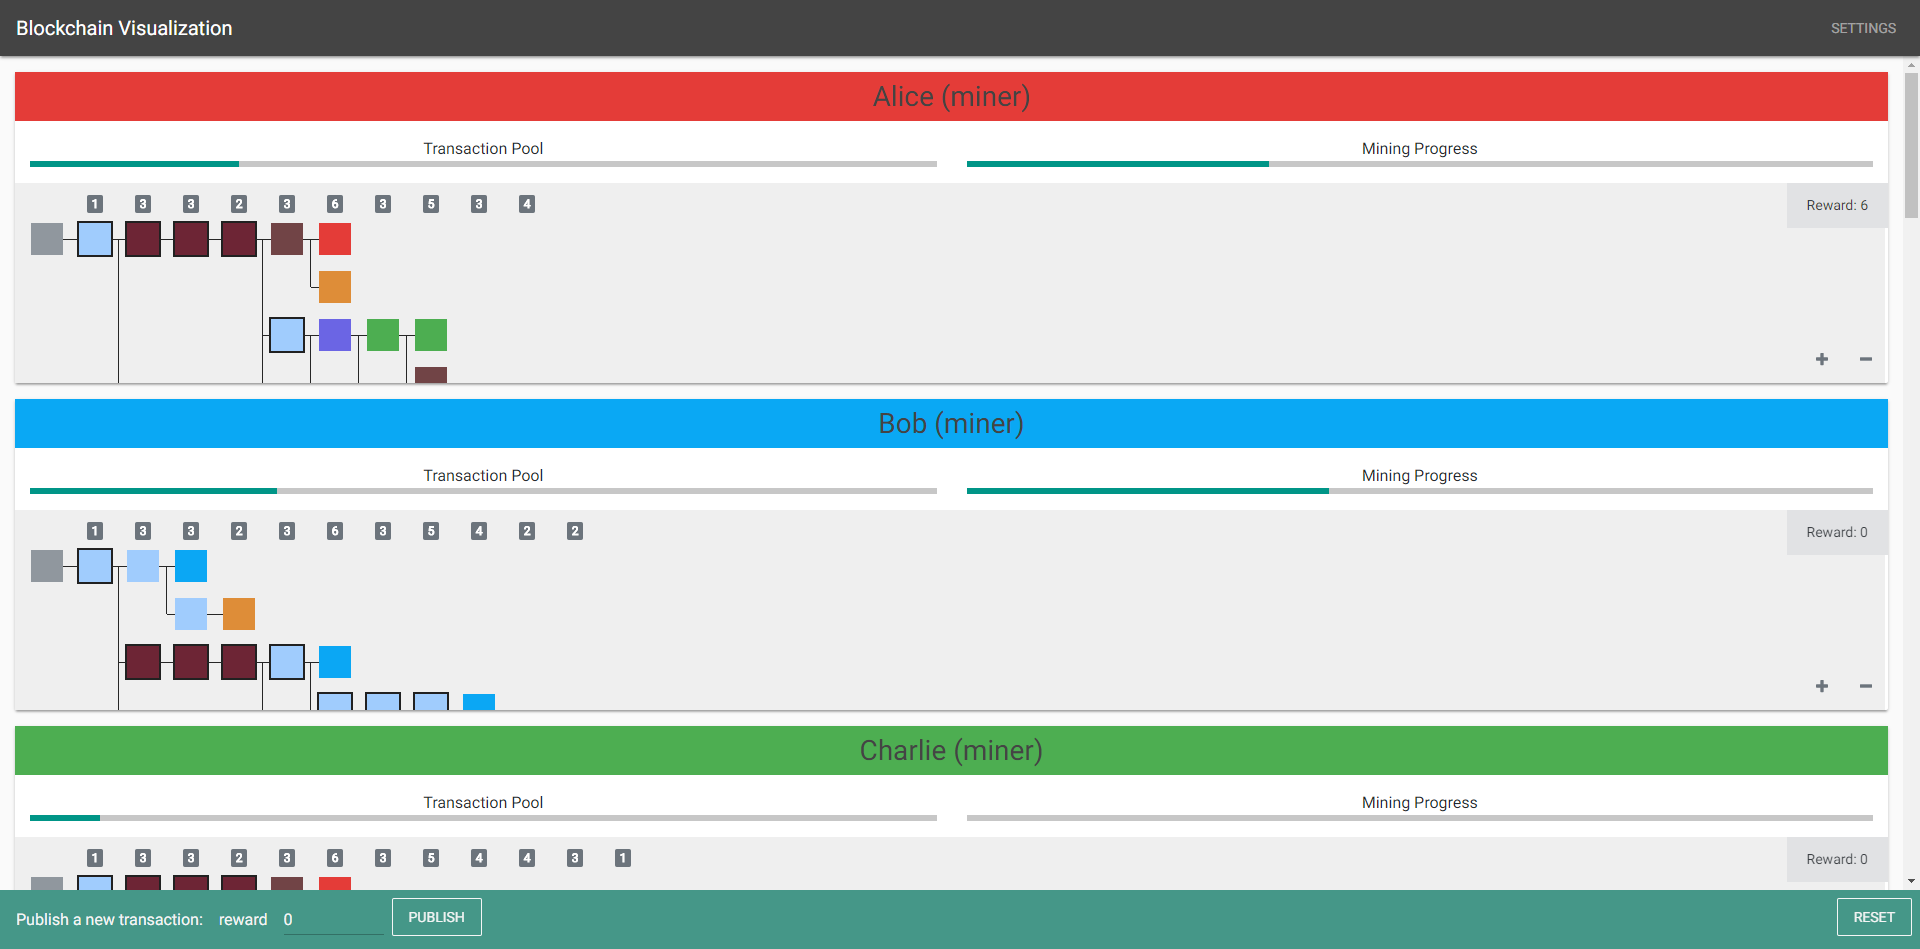
\includegraphics[width=\textwidth]{related_us2}
        \caption{Mining Step 2}
    \end{subfigure}

    \caption{Steps of Mining.}
    \label{fig:steps of mining}
\end{figure}

As we can see in Figure \ref{fig:steps of mining}, the tree structure of the blockchains keeps growing while the mining activities continue. The basic visualization ideas of our project are inspired by a former project called “Kooperative Music Box” \cite{musicbox} which was developed by Fraunhofer Blockchain-Labor. It used shapes and colors to distinguish different blocks and transactions which were generated by different nodes. As a result, in the visualization application, the blocks are represented as squares, and they are chained by lines to form tree structures, and the colorful blocks are generated by different miners.

Our project aims to visualize all the dynamic mining processes that could happen in a blockchain system, with the factors of the network delay and the different mining strategies. This distinguishes our work to all the related works mentioned before. Consequently, our work is worthwhile as a contribution and a trial to the blockchain research area.
